% Chapter 4b
\chapter{Object Reconstruction in the ATLAS Detector} % Chapter title
\label{ch:reconstruction} 

Object reconstruction is the computation-intensive process of turning the signals from the approximately 100 million read-out channels of the ATLAS detector into a collection of particles and jets, the objects with which physics analysis can be performed. This process is complicated, and requires dedicated working groups in the ATLAS experiment that optimize the understanding of each type of object, which must all collaborate to provide a full picture of the events in the detector.

%---------------------------------------------------------------------------------------

\section{Electrons}
\label{sec:reco_electrons}

Electrons are identified through a combination of \ac{ID} and calorimeter measurements. They travel through the tracking system, leaving charge deposits in each layer, then are absorbed by the electromagnetic calorimeter. These two measurements work in conjunction to deliver high resolution measurements of electron momentum from low-\pt, where track curvature gives the most reliable measure of the electron's energy, to high-\pt, where the tracks are almost perfectly straight, but the calorimeter can still provide a reliable measurement. 

In the central region ($|\eta|<2.47$) of the ATLAS detector, electron reconstruction begins with the identification of energy deposits in the electromagnetic calorimeter. The calorimeter clusters are seeded by sliding longitudinal windows, which are measured in units of 0.025 in $\eta$ and $\phi$. 3$\times$5 unit windows are used, which require at least 2.5 \gev~in the window to form a seed \cite{Aad:2011mk}. 

These clusters are matched to \ac{ID} tracks by extrapolating the track to the middle layer of the calorimeter and identifying nearby clusters. If there are multiple tracks associated with a given cluster, tracks with silicon hits are preferentially chosen, and then the track with the smallest $\Delta R$ to the center of the cluster is selected. The track is used to determine the likely direction of bremsstrahlung radiation in the calorimeter, and maximum distance to match a track to a clusters expanded in the $\phi$ direction to account for this radiation.

The calorimeter clusters are then rebuilt in in larger windows, 3$\times$7 in the barrel and 5$\times$5 in the end-caps. An estimate of the energy is made by summing the measured calorimeter energy with estimates of the energy lost before the electron reached the calorimeter, energy outside of the cluster window, and energy not fully deposited in the calorimeter. These estimates are made with parametrized functions determined from a comparison of \ac{MC} and measurements taken by the presampler. 

The momentum is determined though a combination of the calorimeter and track measurements of the electron, while its $\eta$ and $\phi$ are taken from the track at its vertex. The energy of the electron is taken from the calorimeter cluster.

In the forward region, where no tracking is available, electron energy is determined more roughly. Calorimeter cells are formed into variable-sized clusters in regions of significant energy deposition, and the center of the cluster is used to determine angular coordinates of the electron. 

Electrons are identified using an algorithm that uses multivariate analysis to assign a likelihood that a candidate is a true electron based on input from just under twenty different variables. These include track quality, hadronic leakage, and cluster shape, incorporating information from as many subdetectors as possible in its determination of the candidate's quality. Each variable is assigned a \ac{PDF} for true electrons and background processes, and they are collectively used to provide a likelihood value which can be cut on. 

Three levels of identification, \texttt{LHLoose}, \texttt{LHMedium}, and \texttt{LHTight}, are defined with different likelihood cuts, with tighter cuts always a subset of the looser cuts. \autoref{fig:reco_el_eff} gives the efficiencies at each of these working points both for true electrons and for hadrons, which can be misidentified as electrons. Tighter working points have worse efficiencies, but lower misidentification rates. 

\begin{centering}
\begin{figure}[!hbt]
\myfloatalign
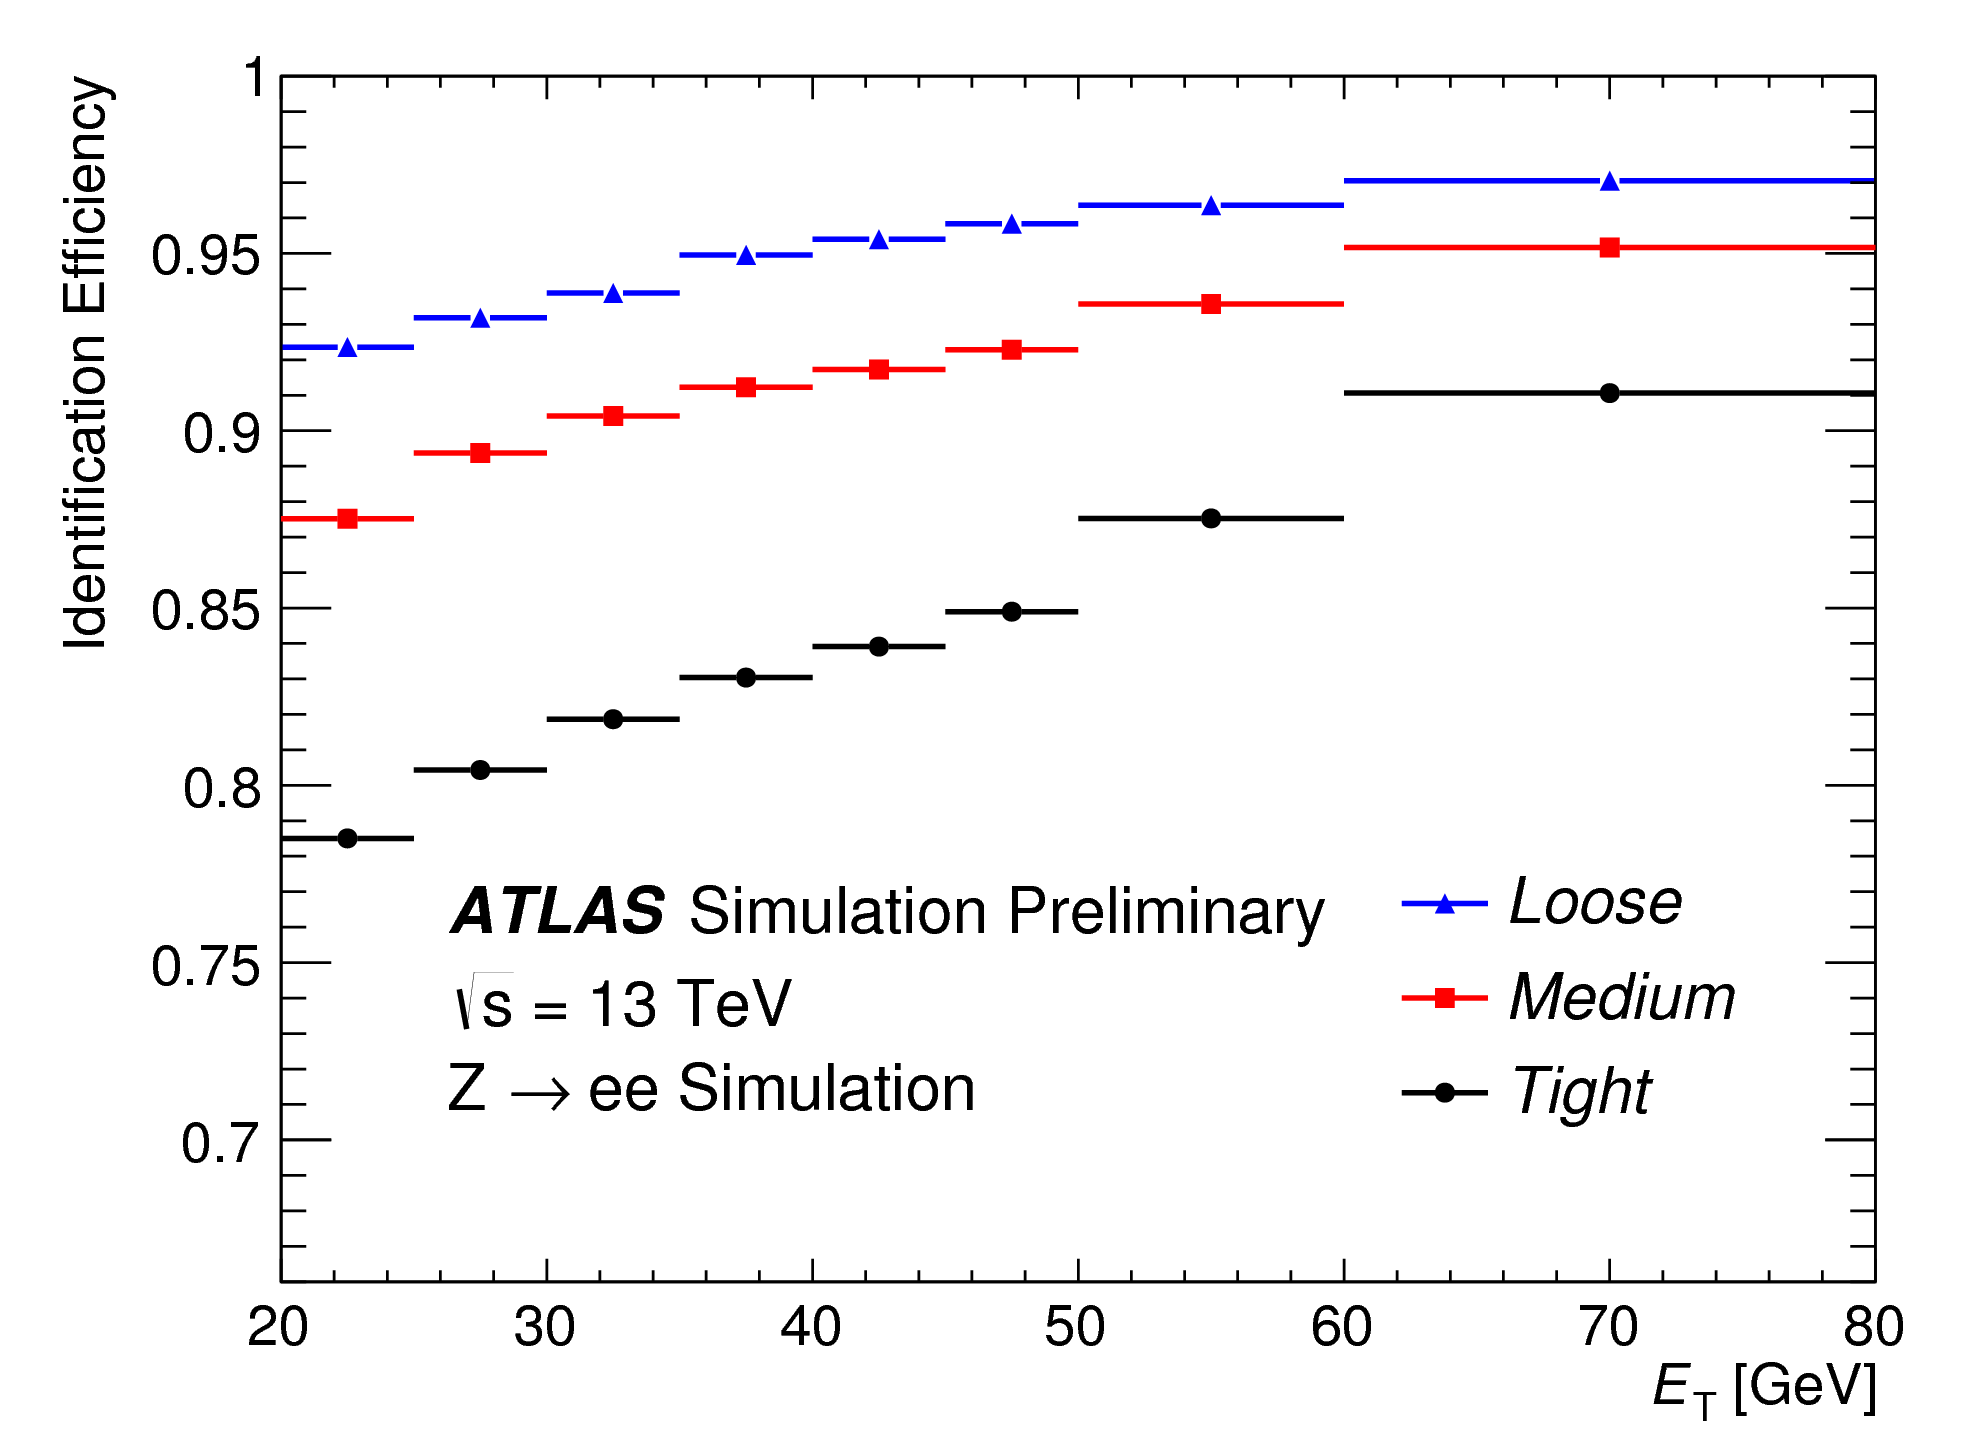
\includegraphics[width=.48\linewidth]{figures/reco/fig_01a.png}
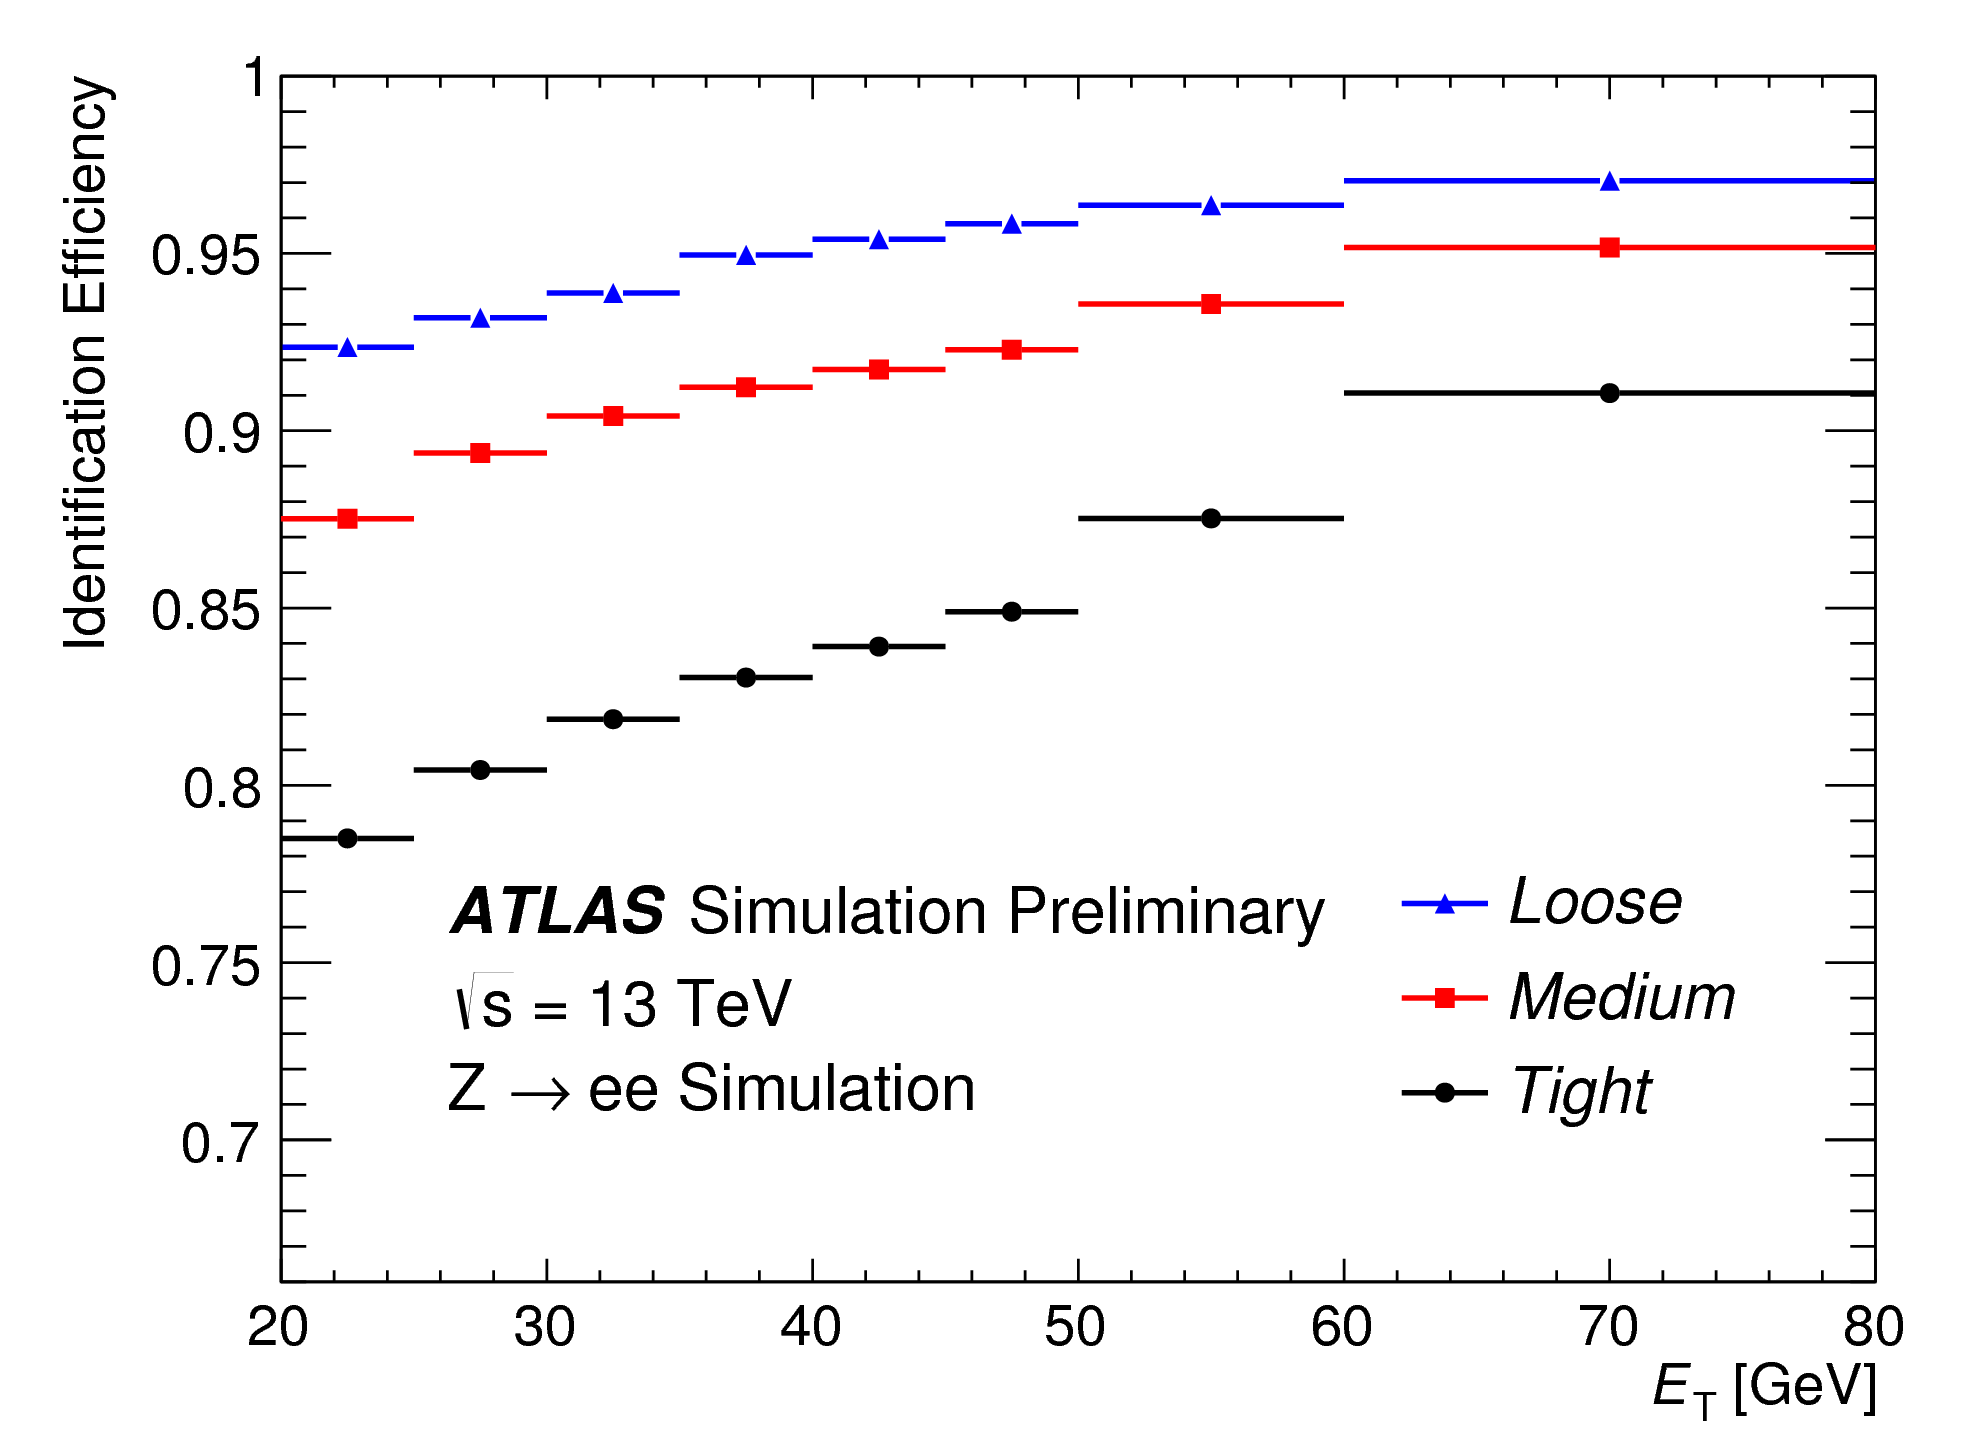
\includegraphics[width=.48\linewidth]{figures/reco/fig_01a.png}
\caption{ Identification efficiencies from \ac{MC} samples for loose, medium, and tight working points. Left is the efficiency for identification of true electrons taken from $Z\rightarrow ee$ \ac{MC}, and right is the efficiency for mis-identification of jets as electrons taken from dijet \ac{MC} \cite{ATLAS-CONF-2016-024}.}
\label{fig:reco_el_eff}
\end{figure}
\end{centering}

\ac{MC} efficiencies can be compared to efficiencies measured in data using the tag-and-probe method, to obtain a \textit{scalefactor}, a correction factor applied to \ac{MC} to better emulate the rates at which electrons are reconstructed and identified. \autoref{fig:reco_el_sf} shows a comparison of the combined reconstruction and identification efficiencies in data and \ac{MC}, with the resulting scalefactors also displayed as the ratio. 

\begin{centering}
\begin{figure}[!hbt]
\myfloatalign
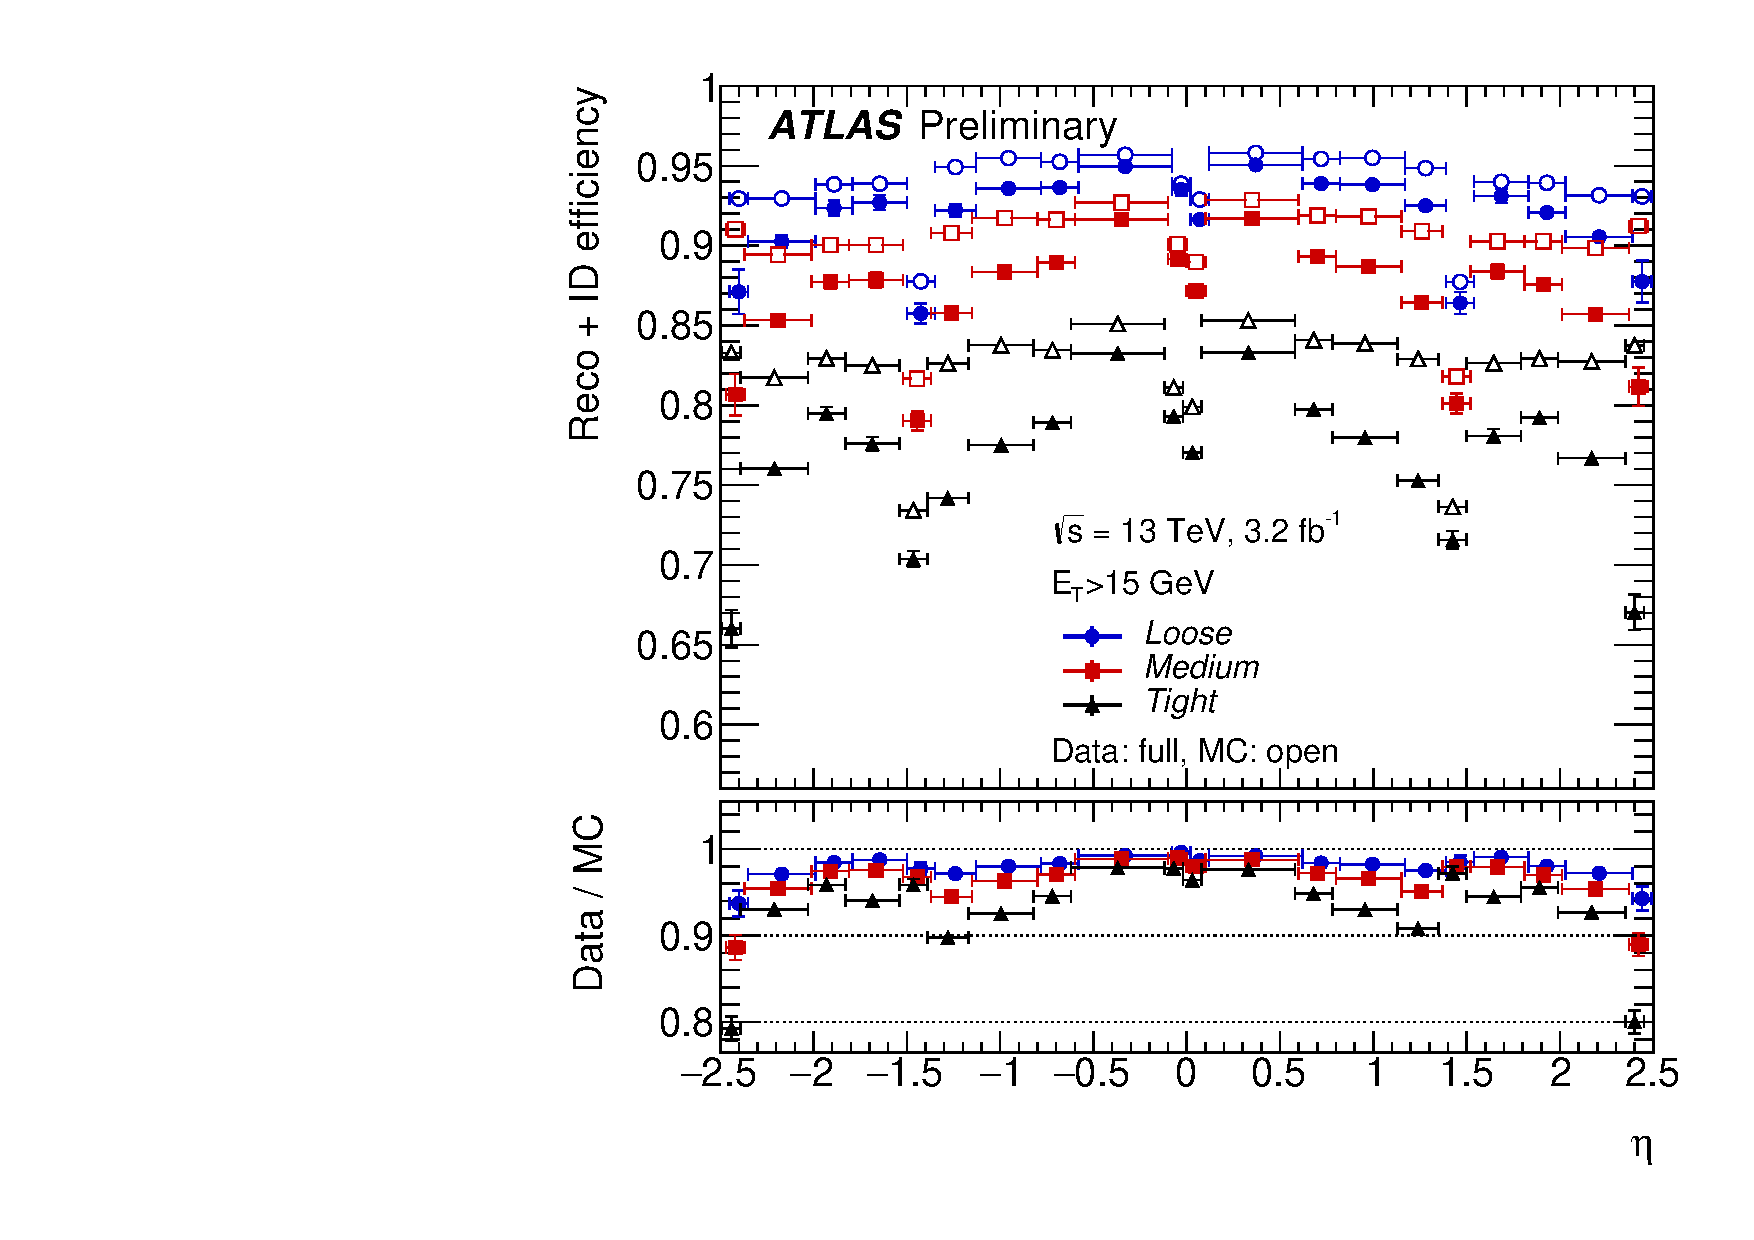
\includegraphics[width=.90\linewidth]{figures/reco/fig_14b.pdf}
\caption{ Combined electron reconstruction and identification efficiencies measured as a function of $\eta$ for data (using the tag-and-probe method on $Z\rightarrow ee$ events) and $Z\rightarrow ee$ \ac{MC}. Distributions include all electrons with \et > 15 \gev. \cite{ATLAS-CONF-2016-024}.}
\label{fig:reco_el_sf}
\end{figure}
\end{centering}

Electrons can also have \textit{isolation} requirements, cuts on nearby calorimeter activity or tracks. Isolation variables are primarily used to reject non-prompt leptons, which can be produced in heavy flavor hadron decays, converted photons, and misidentified hadrons. Cuts are made on the amount of nearby calorimetric energy and sum of the \pt of nearby tracks relative to the electron's energy, forming a series of working points. Fixed cut working points, which specify the relative fraction to cut on, can be used, but efficiency targeted working points are more popular. These include \texttt{Tight} and \texttt{Loose} working points, which operate at 95 and 98\% efficiency respectively, and working points that target tighter efficiencies at higher electron \pt, \texttt{Gradient} and \texttt{GradientLoose}. These working points each have 99\% efficiency for electrons with \pt > 60 \gev, but 90 and 95\% efficiencies at 25 \gev. 

\section{Photons}
\label{sec:reco_photons}

The reconstruction of photons is performed in parallel to electron reconstruction. Seed clustering is performed, and tracks are matched to these clusters, as in the case of the electron reconstruction described in \autoref{sec:reco_electrons}. 

Photons can be converted to electron-positron pairs in the \ac{ID}, leaving a pair of tracks, or they can pass through without conversion, leaving no tracks behind. As a consequence, calorimeter clusters resulting from photons can have no tracks associated with them, two tracks, or one track, in the case that one of the conversion tracks is not reconstructed. The reconstruction software attempts to identify all these scenarios and differentiate these processes from electron and hadron deposits \cite{1606.01813}.

Two-track clusters are required to consist of two oppositely charged tracks that emerge from a conversion vertex running parallel to one another. A likelihood that these are from electrons is determined using the high threshold hits in the \ac{TRT}, and cuts on this likelihood are made for tracks with and without silicon hits, 10 and 80\% respectively. The tracks are fit to produce the conversion vertex, and quality cuts are made, such as requiring that conversion vertices within the silicon volume correspond to tracks with silicon hits. 

Single track clusters occur most often from conversions in the outermost layers of the \ac{ID}, and are more difficult to reconstruct. Tracks are typically lost because the coverted electron is too low \pt to be reconstructed, or because the two tracks are so close together that they're identified as a single track. The single track is required to have at least a 95\% electron likelihood, and must not have a hit in the innermost layer of the pixel detector. The conversion vertex is defined as the first hit of the track. 

These conversion vertices are extrapolated to the calorimeter and matched to clusters. If multiple vertices are matched to a single cluster, preference is given to vertices with double tracks, silicon hits, and finally to tracks closest to the interaction point. 

Any cluster with neither a conversion vertex or a track reconstructed to it is identified as an unconverted photon. Clusters with conversion vertices are reconstructed as photons unless the cluster is also associated with an electron and the tracks associated with the cluster don't match the tracks associated with the conversion vertex. Single track clusters associated with electrons are instead identified as photons if the track has no silicon hits. 

The photon's energy is determined in 3$\times$5 (3$\times$7) windows for unconverted (converted) photons in the barrel, where the window is expanded to compensate for the increased spread of energy from the conversion products. In the endcap, the 5$\times$5 window is used in all cases. Like the electrons, the calibration of the photon's energy accounts for energy loss before the calorimeter, as well as energy deposited outside the cell and beyond the electromagnetic calorimeter.

Photon identification is performed in the range $|\eta|<2.37$ using a series of cuts on the shape of the shower in the electromagnetic calorimeter, as well as the amount of additional energy deposited in the hadronic calorimeter. Photons in the the so called \textit{crack} region of the calorimeter ($1.37<|\eta|<1.52$), where a discontinuity prevents accurate assessment of photon energy, are rejected. The identification has a \texttt{Loose} and a \texttt{Tight} working point. The \texttt{Tight} working point is used most often, and has an identification efficiency of 53–64\%(47–61\%) for unconverted (converted) photons with \et = 10 \gev~and 88–92\% (96–98\%) for photons with \et $\geq$ 100 \gev \cite{ATL-PHYS-PUB-2016-014}. Efficincies as a function of \pt measured in the 2016 data and compared to \ac{MC} can be seen in \autoref{fig:reco_photon_eff}.

\begin{centering}
\begin{figure}[!hbt]
\myfloatalign
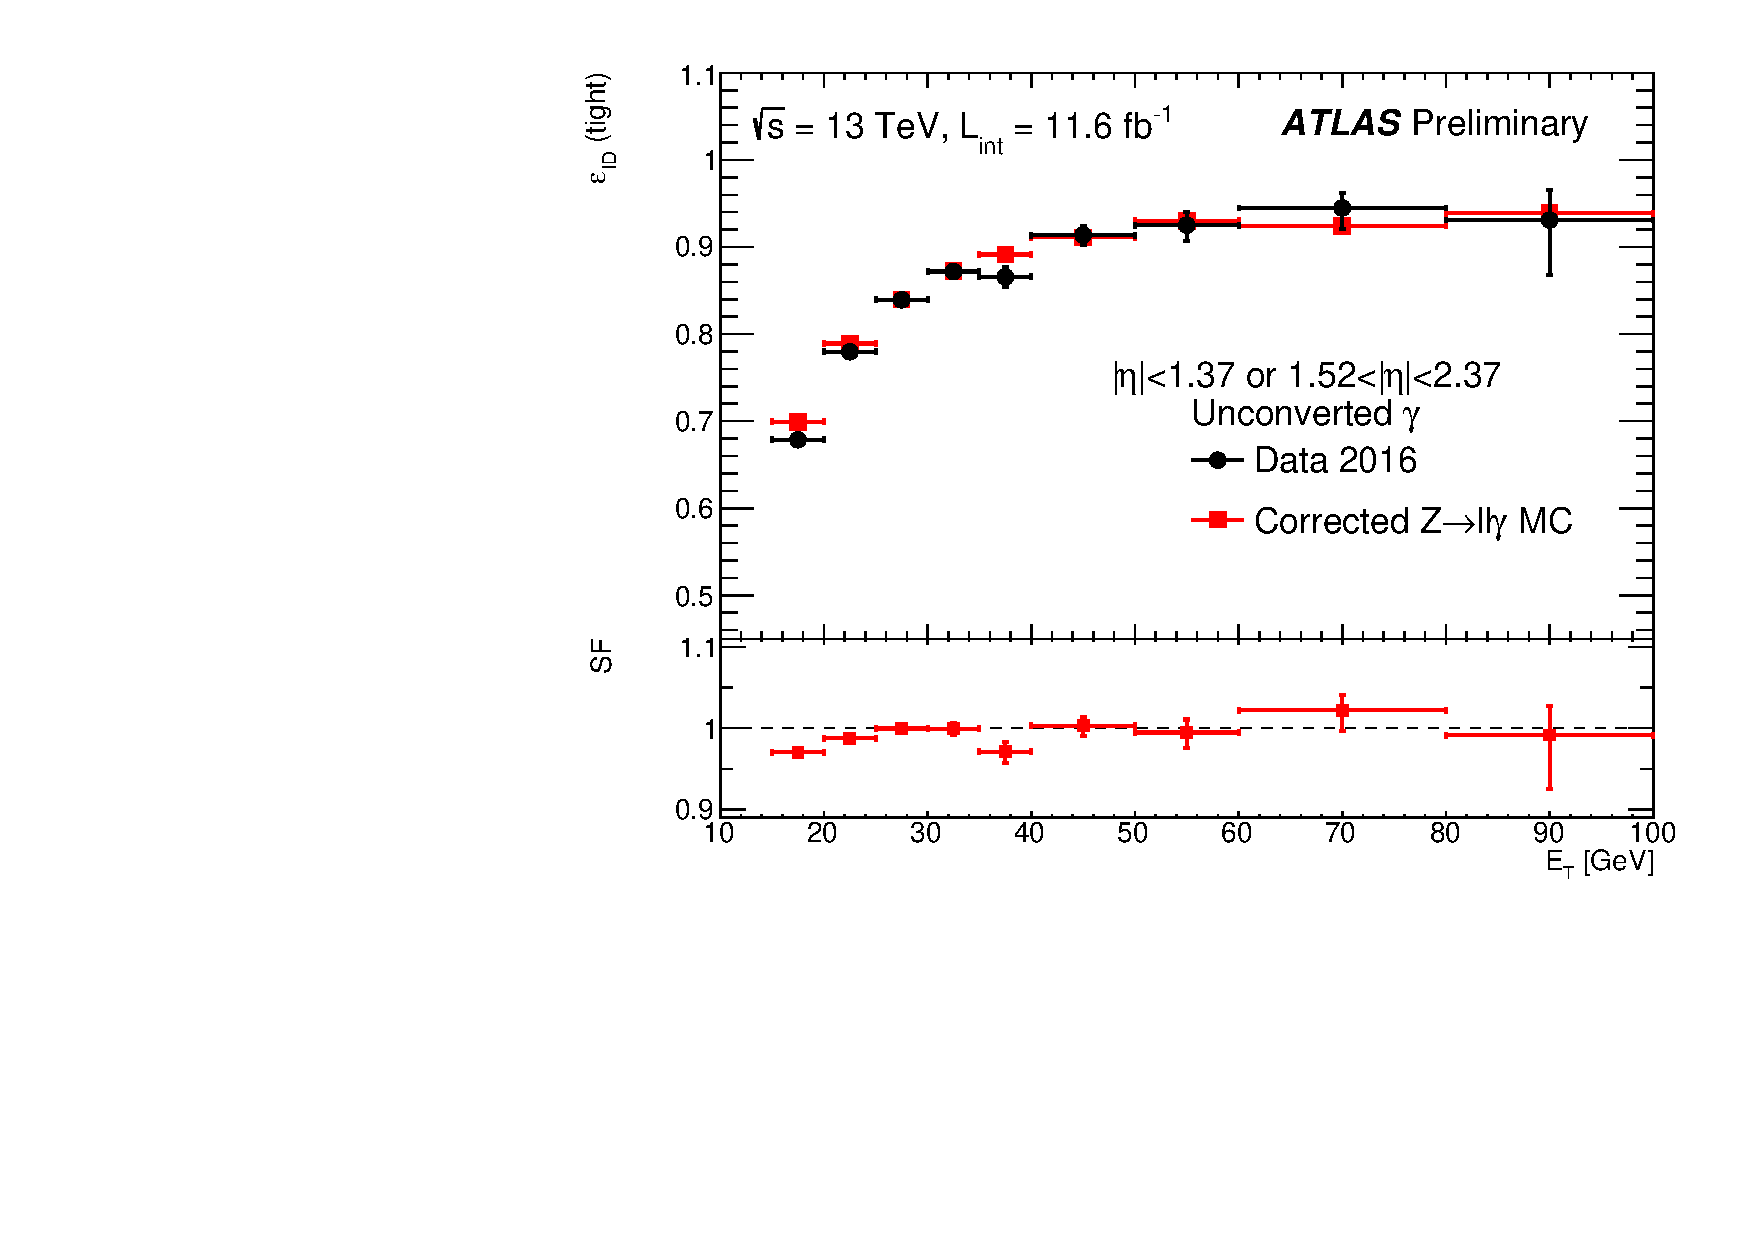
\includegraphics[width=.48\linewidth]{figures/reco/photon_fig_01.pdf}
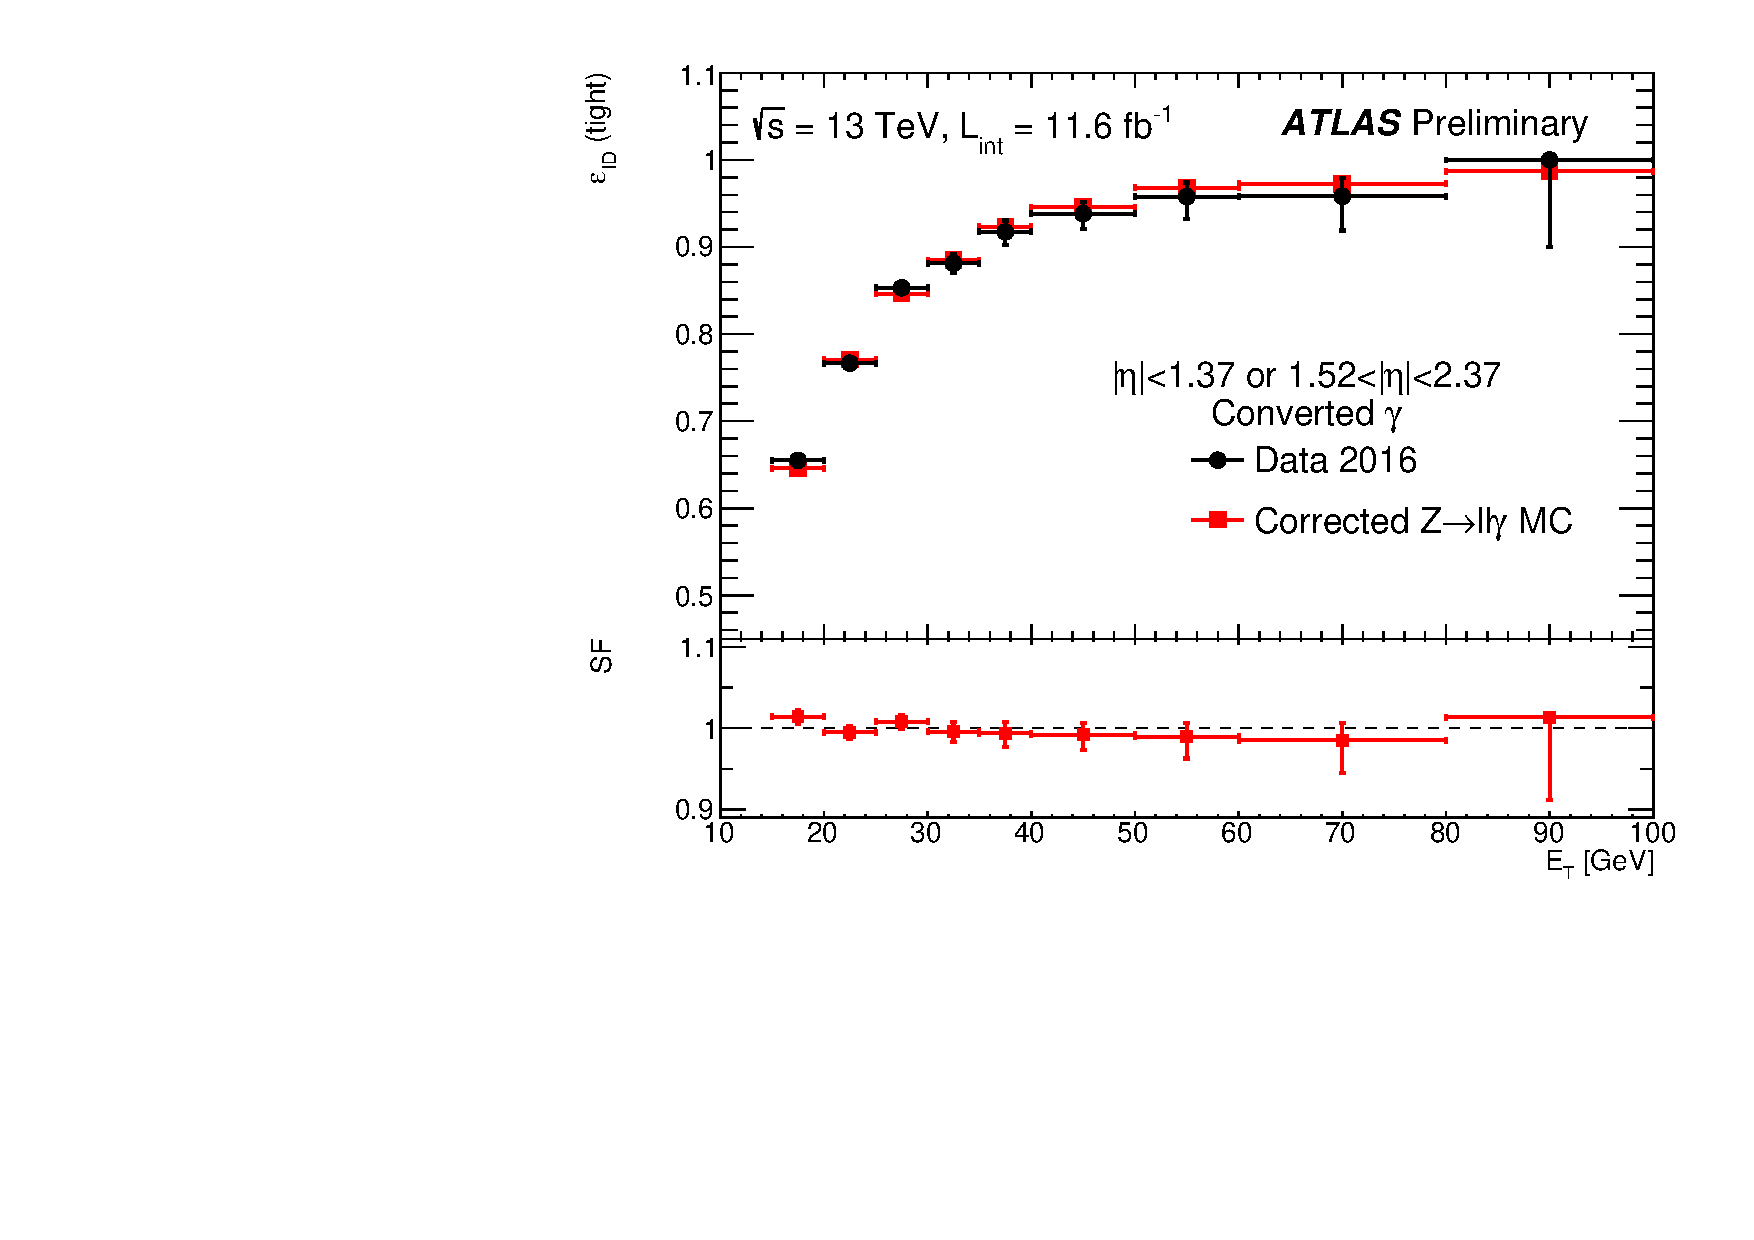
\includegraphics[width=.48\linewidth]{figures/reco/photon_fig_02.pdf}
\caption{ Comparison of tight identification efficiency measurements from data and $Z\rightarrow \ell\ell\gamma$ \ac{MC} for unconverted (left) and converted (right) photons, with an inclusive $\eta$ election. The bottom of each figure shows the ratio of data and \ac{MC} efficiencies. \cite{EGAM-2016-003}.}
\label{fig:reco_photon_eff}
\end{figure}
\end{centering}

Photon isolation, like electron isolation, can be determined as the combination of nearby calorimeter deposits and tracks. Fixed cuts on the isolation as a fraction of photon energy is typically used. A working point called \texttt{FixedCutTight} reconstructs the amount of calorimeter energy (excluding that of the photon) in a cone of $\Delta R  = 0.4$ around the photon and the amount of energy from the sum of track \pt in a cone of $\Delta R = 0.2$. Defined relative to the photon's \pt, this working point includes photons with calorimetric isolation less than 0.022\pt + 2.45 \gev~and track isolation less than 0.05\pt \cite{isolation}. 

\section{Muons}
\label{sec:reco_muons}

Muon reconstruction is performed independently in the \ac{ID} and the \ac{MS}, then the two measurements are combined when possible \cite{1603.05598}. The \ac{ID} reconstruction is performed using the tracking mechanism over the $|\eta|<2.5$ range. As with electrons, hits in the layers of the \ac{ID} are fit to tracks, a process described in more detail in \autoref{sec:NN}.

The \ac{MS} track reconstruction begins with a search in each muon chamber for patterns of hits consistent with a track, called \textit{segments}. The \ac{MDT} chamber hits are fit to a straight line, and nearby \ac{RPC} and \ac{TGC} chambers provide the coordinate orthogonal to the magnetic curvature for these hits. The \ac{CSC} segments are required to be loosely consistent with a track originating from the interaction point. 

These segments are then fit together, starting from the middle layers of the \ac{MS}, with track quality requirements on the resulting combinations based on the $\chi^2$ of the fits. Tracks must have at least two segments, except in the transition region between the barrel and endcap, where a single high quality segment can qualify as a track. Shared segments are allowed in the initial reconstruction, but after the combination, tracks with shared segments and low quality fits are removed.    

These \ac{MS} tracks are then combined with measurements from other parts of the ATLAS detector. The best quality muons are combined muons, which have \ac{ID} and \ac{MS} tracks associated to them, the hits of which are re-fit to form a combined track. \ac{MS} hits can be added or removed at this stage based on their consistency with the new track. Other types of muons exist, including extrapolated muons, which have only \ac{MS} tracks that are consistent with the interaction point, calorimeter-tagged muons, which combine an \ac{ID} track with a calorimeter deposit consistent with a muon, and segment-tagged muons, which combine an \ac{ID} track with a segment in the \ac{MS}. Muons with shared \ac{ID} tracks are not allowed, with preference given to combined muons, then calorimeter-tagged muons, and lastly segment-tagged muons. 

There are four muon identification working points for muons: \texttt{Loose}, \texttt{Medium}, \texttt{Tight}, and \texttt{High-p$_\texttt{T}$}. These working points all have different efficiencies for the identification of muons, balanced against the mis-identification of hadrons. One of the key variables for their discrimination is $q/p$ significance, which quantifies the consistency between the \ac{ID} and \ac{MS} measurements of momentum. The $\chi^2$ of the combined fit is also an important discriminator. 

The \texttt{Loose}, \texttt{Medium}, and \texttt{Tight} efficiencies are inclusive, with all \texttt{Tight} muons passing the \texttt{Medium} requirements, for example. The \texttt{Loose} requirement includes all types of muons, but allows muons without \ac{MS} tracks only in the $\eta<0.1$ range where coverage of the \ac{MS} is incomplete. The \texttt{Medium} working point includes only combined and extrapolated muons, and is the default for most ATLAS analyses. Extrapolated muons are allowed only in the $\eta$ range outside the \ac{ID} tracking system, a region often excluded by analyses because of the decreased quality. For the combined muons, at least three hits in at least two \ac{MDT} layers are required (except in the $\eta<0.1$ region) and a $q/p$ significance cut is made to reduce backgrounds. Even with the reduced requirements at low $\eta$, there is a drop in efficiency in this region, as shown in \autoref{fig:reco_muon_eta}. The \texttt{Tight} working point additionally cuts on $\chi^2$ and $p'$, another variable that quantifies the discrepancy between \ac{ID} and \ac{MS} \pt measurements. 

\begin{centering}
\begin{figure}[!hbt]
\myfloatalign
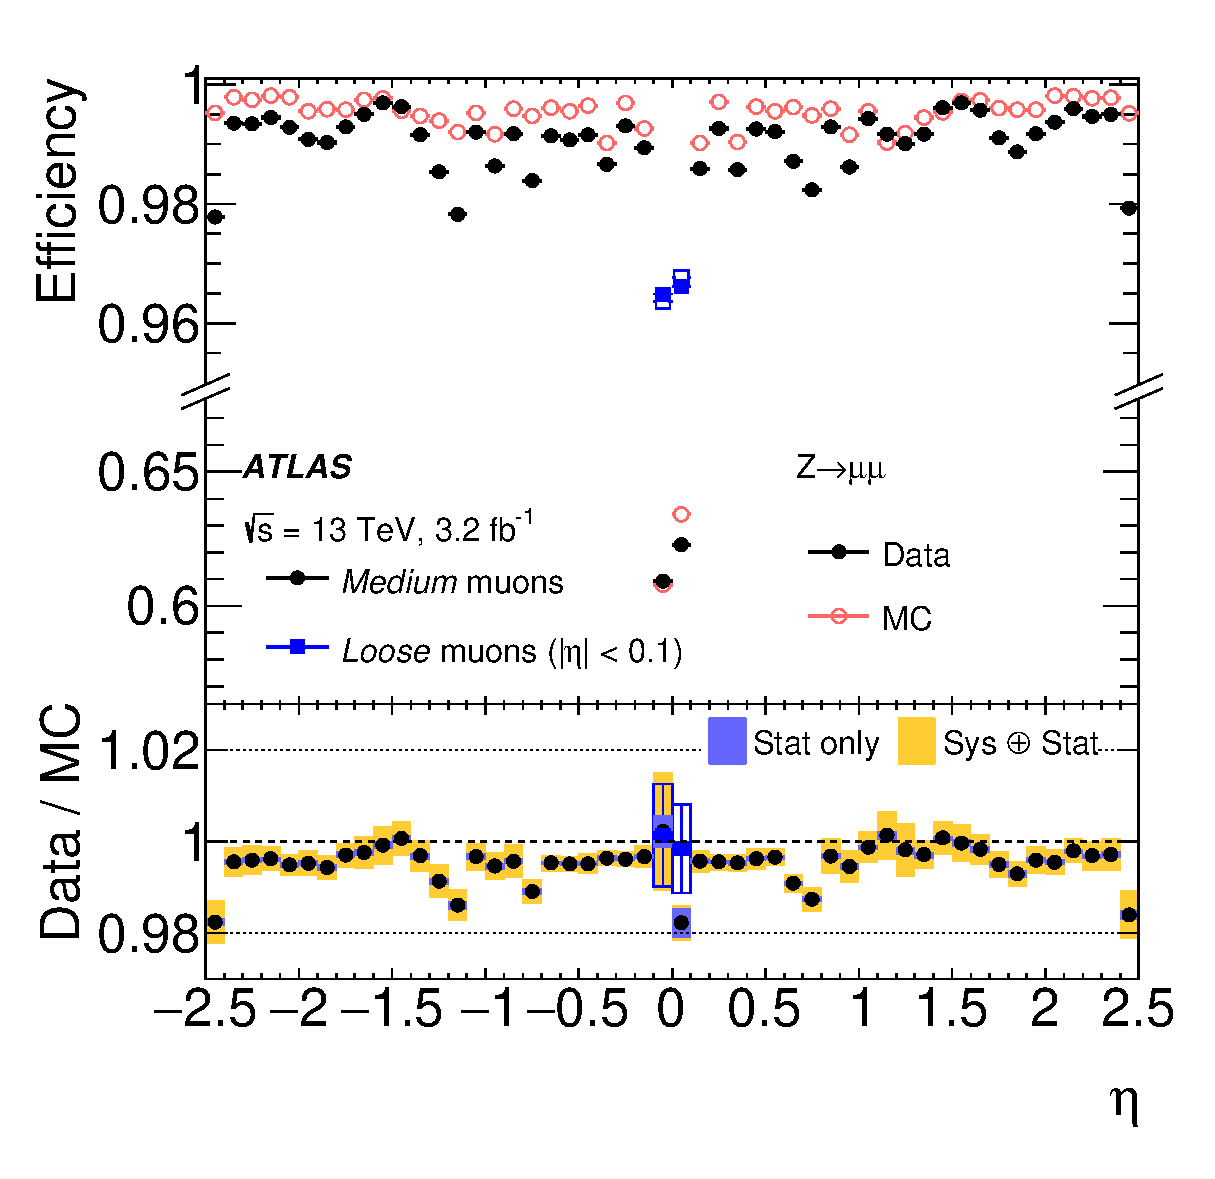
\includegraphics[width=.9\linewidth]{figures/reco/fig_03a.eps}
\caption{Muon reconstruction efficiency for the \texttt{Medium} working point measured with $Z\rightarrow\mu\mu$ events in data using the tag-and-probe method and in \ac{MC} as a function of $\eta$. The ratio between the two is shown at the bottom. \cite{1603.05598} }
\label{fig:reco_muon_eta}
\end{figure}
\end{centering}


The \texttt{High-p$_\texttt{T}$} working point is designed to maximize efficiency for high-\pt muons, at the cost of lower efficiencies for low-\pt muons. Muons must have at least three \ac{MDT} hits in three layers, which decreases efficiency but gives greatly improved \pt resolution. In addition, some regions of the \ac{MS} with low-performing chambers are vetoed to cut down on mismeasurement. Compared to the default working point these muons have much lower efficiency: 78\% (90\%) for \texttt{High-p$_\texttt{T}$} muons compared to 96\% (96\%) for \texttt{Medium} in the \pt range of 4-20 \gev~(20-100 \gev). The efficiency as a function of $\eta$ for this working point can be seen in \autoref{fig:reco_muon_eta_highpt}, where the efficiency loss due to the of vetoing of some chambers is especially apparent.

\begin{centering}
\begin{figure}[!hbt]
\myfloatalign
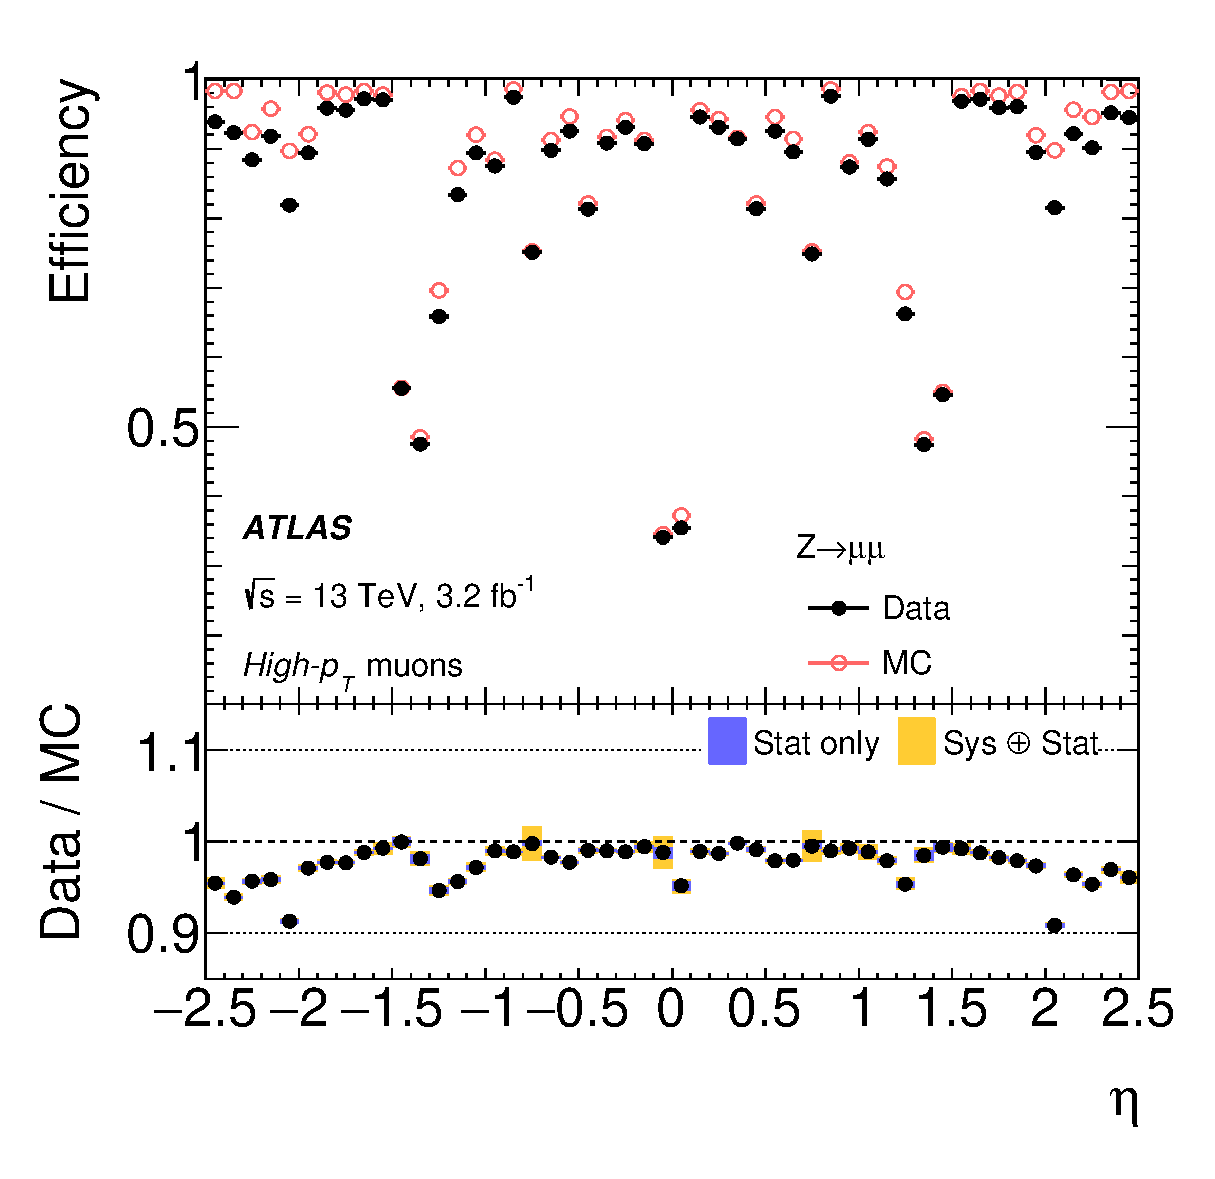
\includegraphics[width=.9\linewidth]{figures/reco/fig_03c.eps}
\caption{Muon reconstruction efficiency for the \texttt{High-p$_\texttt{T}$} working point measured with $Z\rightarrow\mu\mu$ events in data using the tag-and-probe method and in \ac{MC} as a function of $\eta$. The ratio between the two is shown at the bottom. \cite{1603.05598} }
\label{fig:reco_muon_eta_highpt}
\end{figure}
\end{centering}

The most common isolation selection for muons is designed in the same way as the electron isolation, and also called \texttt{GradientLoose}. It is constructed such that muons with \pt of 25 \gev~have an efficiency of 95\%, and muons with \pt of 60 \gev~have an efficiency of 99\%. 

\section{Jets}
\label{sec:reco_jets}

Jets are the most complicated objects to reconstruct in the ATLAS detector because each jet is an assembly of many hadronic particles. In contrast to a lepton, whose reconstructed energy can easily be compared to its true energy from simulation, even a jet's true energy is ambiguous, and is dependent on the choice of the jet's definition. The standard jet reconstruction algorithm used in the ATLAS experiment is called anti-$k_t$ \cite{Cacciari:2008gp}. 

This algorithm begins with calorimeter clusters defined by topologically connected cells with energy deposits significantly higher than the noise background. In fact, there are two collections of these clusters, one with cluster energies calibrated for electromagnetic showers (\acs{EM}), and another calibrated to hadronic showers. The second uses a method called \ac{LCW}, which first classifies a cluster as electromagnetic or hadronic based on the energy density and the shower depth, then applies a calibration according to the classification for each cluster.

The anti-$k_t$ algorithm is then applied to these clusters, which begins with the highest energy cluster and groups it with nearby clusters according to the distance measure

\begin{equation}
d_{ij} = min(k^{-2}_{ti}, k^{-2}_{tj}) \frac{\Delta_{ij}^2}{R^2}
\end{equation}

where $R$ is the algorithm's radius parameter, typically set to 0.4, $\Delta$ gives the angular separation of the two clusters, and $k_t$ is the transverse momentum associated with the cluster. Clusters are added to the jet within the cone radius, then the axis of the jet is reassessed. This process is repeated until a stable jet is produced. The inverse dependence on the $k_t$ of the cluster produces jets with energetic cores and softer edges, which matches the expectation from a hadronic shower. In addition it is infrared and collinear safe, with neither soft emission or collinear tracks altering the reconstruction of the jet. 

A series of calibrations are then applied to these jets. The first is to correct for additional hadronic energy due to pile-up, shown in \autoref{fig:reco_jet_nvtx}. To do this, a correction taken from \ac{MC} and parametrized in terms \pt and $\eta$, as well as the number of primary vertices in the event as well as the average number of vertices, which makes correction for out-of-time pile-up possible. Next, jets are corrected to have their origin at the primary vertex instead of the center of the ATLAS detector. After that, the jets are corrected based on jet energy and $\eta$ dependent \ac{JES} factors derived from \ac{MC}. \autoref{fig:reco_JES} shows the energy response, the inverse of these factors, for \ac{EM} jets. Lastly, some regions of the detector have been shown to have a bias in $\eta$ measurement of jets, and this is accounted for. 

\begin{centering}
\begin{figure}[!hbt]
\myfloatalign
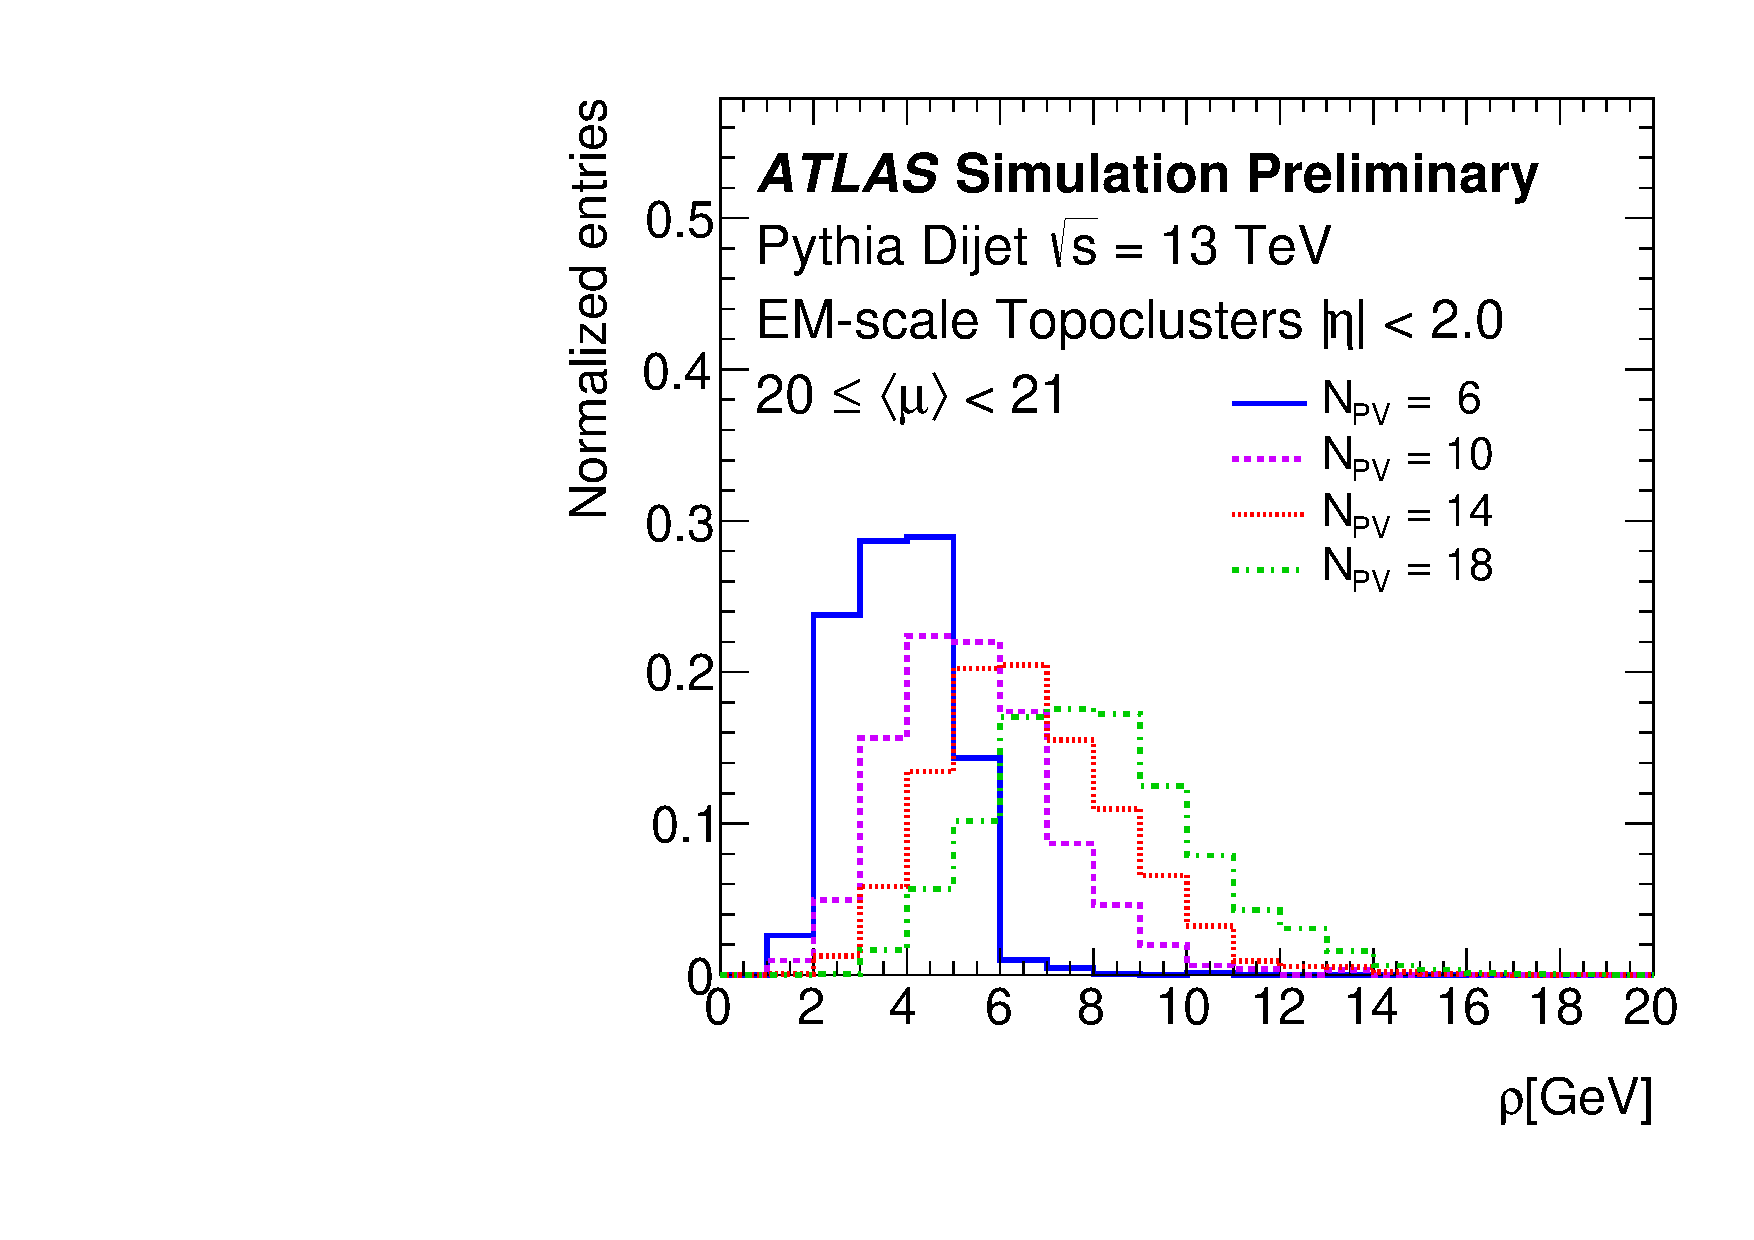
\includegraphics[width=.9\linewidth]{figures/reco/fig_02.pdf}
\caption{ Distribution of event \pt density, $\rho$, taken from \ac{MC} dijets for different numbers of primary vertices. \cite{ATL-PHYS-PUB-2015-015} }
\label{fig:reco_jet_nvtx}
\end{figure}
\end{centering}

\begin{centering}
\begin{figure}[!hbt]
\myfloatalign
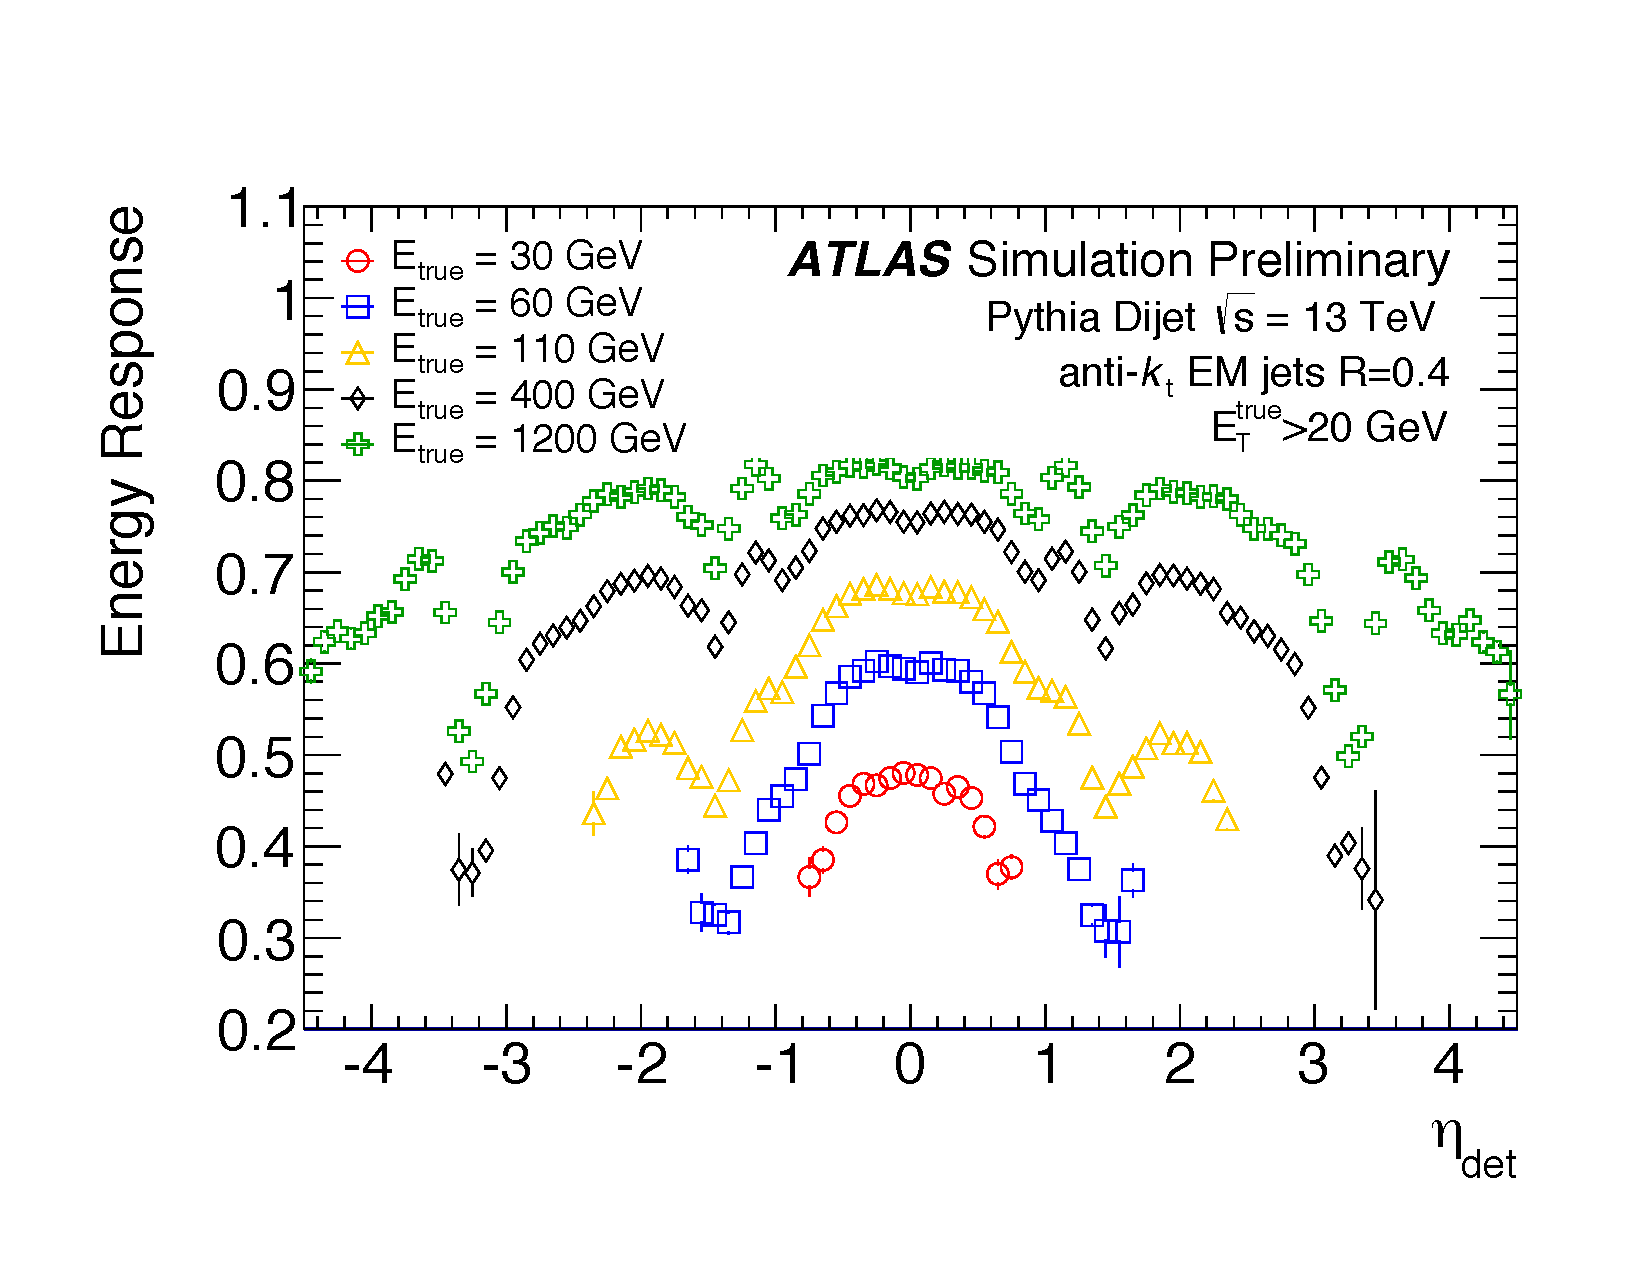
\includegraphics[width=.9\linewidth]{figures/reco/fig_04a.pdf}
\caption{ Energy response as a function of energy and $\eta$ for \ac{EM} jets in dijet \ac{MC}. \cite{ATL-PHYS-PUB-2015-015} }
\label{fig:reco_JES}
\end{figure}
\end{centering}

In addition to correcting for additional energy due to pile-up, it is necessary to reject reconstructed jets that come from pile-up vertices. To accomplish this, a multivariate alogrithm called \ac{JVT} was created which builds upon an older method, \ac{JVF} \cite{ATLAS-CONF-2014-018}. The original method vetoed jets by summing the total \pt of associated tracks and assessing the fraction of that \pt that came from tracks associates with the event's primary vertex. This fraction decreases with higher pile-up, making the construction of an explicit cut difficult in pile-up varying conditions. \ac{JVT} improved on the method by producing a pile-up corrected \ac{JVF} variable and including it in the inputs of the tagger with other variables including a similar variable, where the sum of track \pt is replaced with the calibrated jet \pt. \autoref{fig:reco_jvt} shows the efficiency and fake rate for the two methods, demonstrating \ac{JVT}'s superior ability to reject pile-up jets even in events with many pile-up vertices.

\begin{centering}
\begin{figure}[!hbt]
\myfloatalign
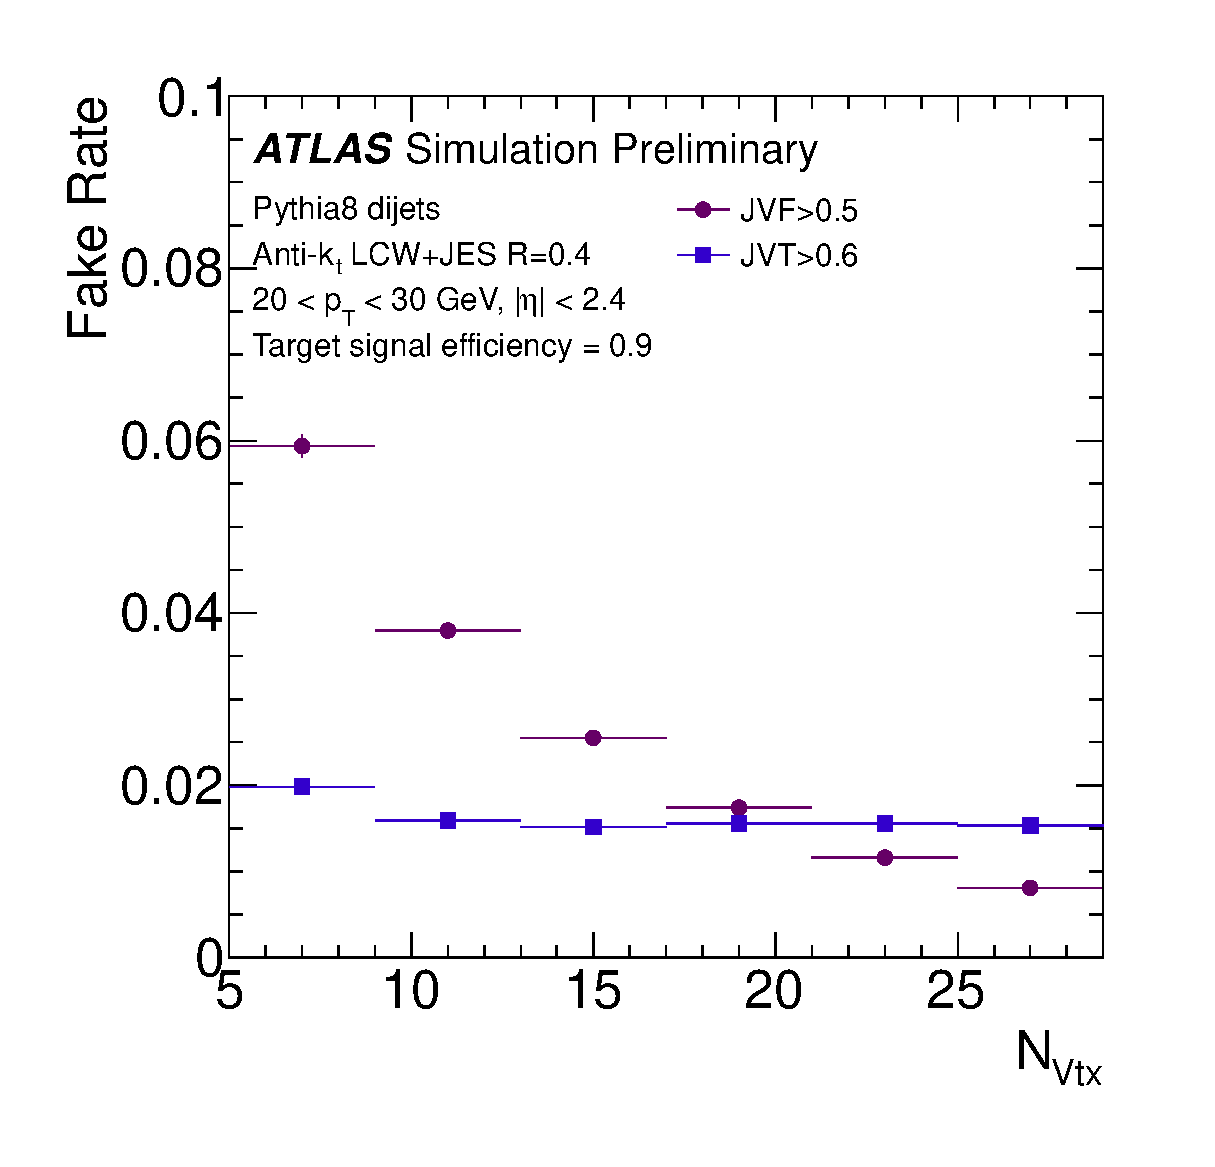
\includegraphics[width=.48\linewidth]{figures/reco/jvt_fig_06b.eps}
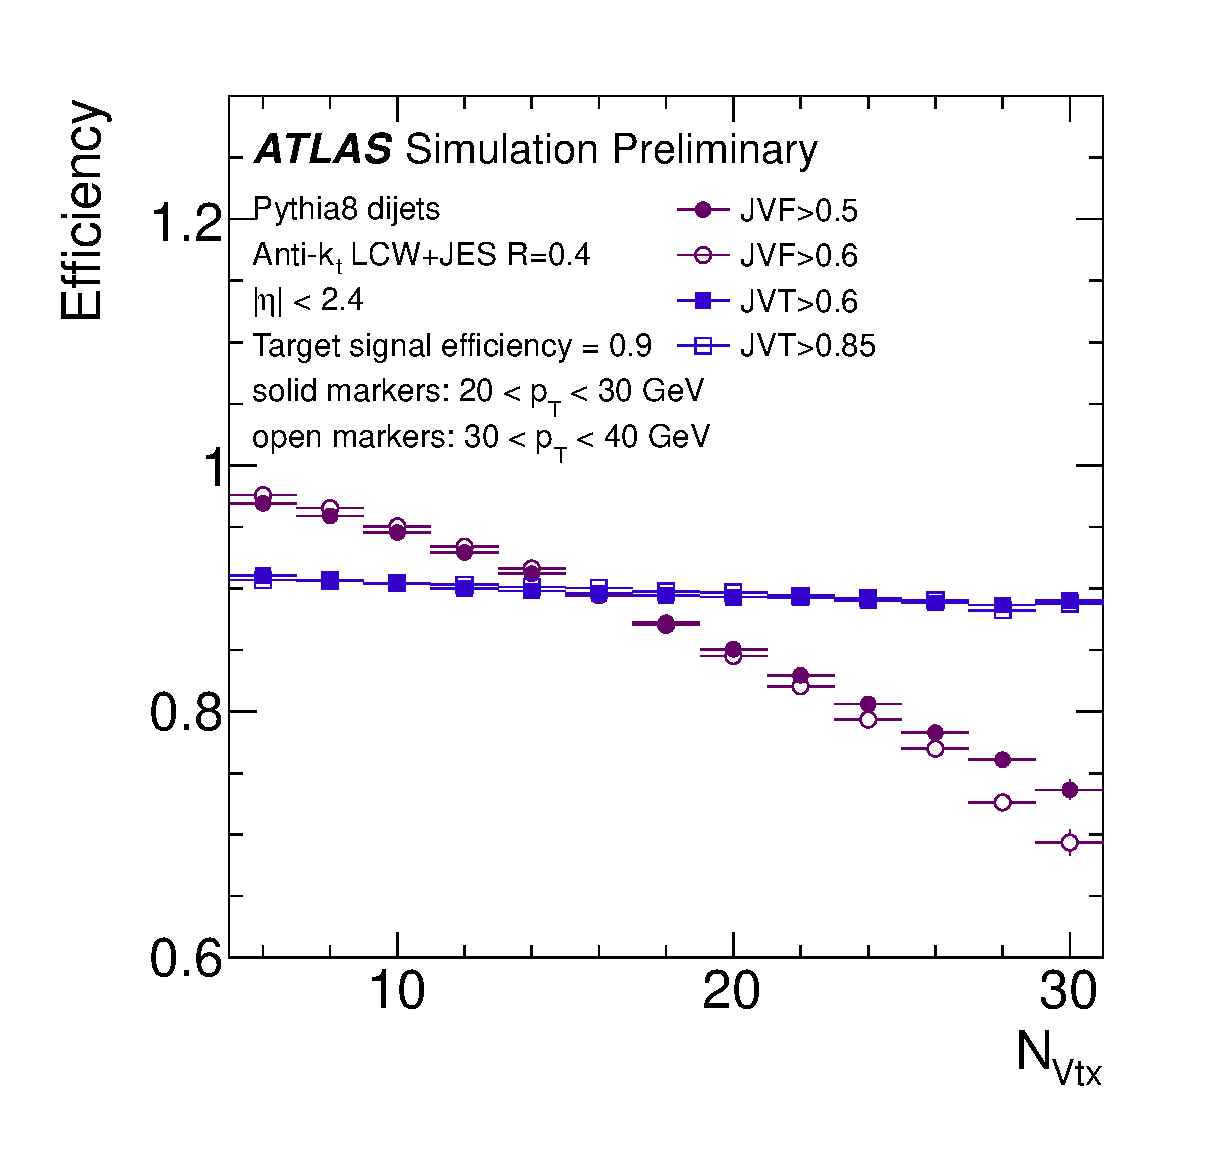
\includegraphics[width=.48\linewidth]{figures/reco/jvt_fig_07a.eps}
\caption{ Dijet \ac{MC} distributions of the number of pile-up jets passing the \ac{JVT} and \ac{JVF} cuts (left) and the efficiency for jets from the primary vertex (right) as a function of number of primary vertices in the event \cite{ATLAS-CONF-2014-018}. }
\label{fig:reco_jvt}
\end{figure}
\end{centering}

It is possible to differentiate jets resulting from $b$-hadron decays from other jets due to the non-negligible lifetimes of the hadrons. Many \ac{BSM} processes preferentially produce $b$ quarks, as does any process involving top quarks, so this identification can be very useful for targeting specific decays in many analyses. Multivariate techniques are used to identify secondary vertices using the \ac{ID}\cite{ATL-PHYS-PUB-2015-022}. In ATLAS, separate algorithms are used to identify jets with tracks with significantly non-zero impact parameters, tracks that reconstruct a secondary vertex, and tracks that can be identified with a chain of vertices beginning with the primary vertex. This information is fed into a boosted decision tree called \texttt{MV2c20}, which outputs a discriminant shown in \autoref{fig:reco_mv2}. Using this discriminant, a working point is chosen such that $b$-jets can be identified with a 70\% efficiency, with mis-identification rates at around 12\% for $c$-jets and 0.2\% for light-flavor jets.

\begin{centering}
\begin{figure}[!hbt]
\myfloatalign
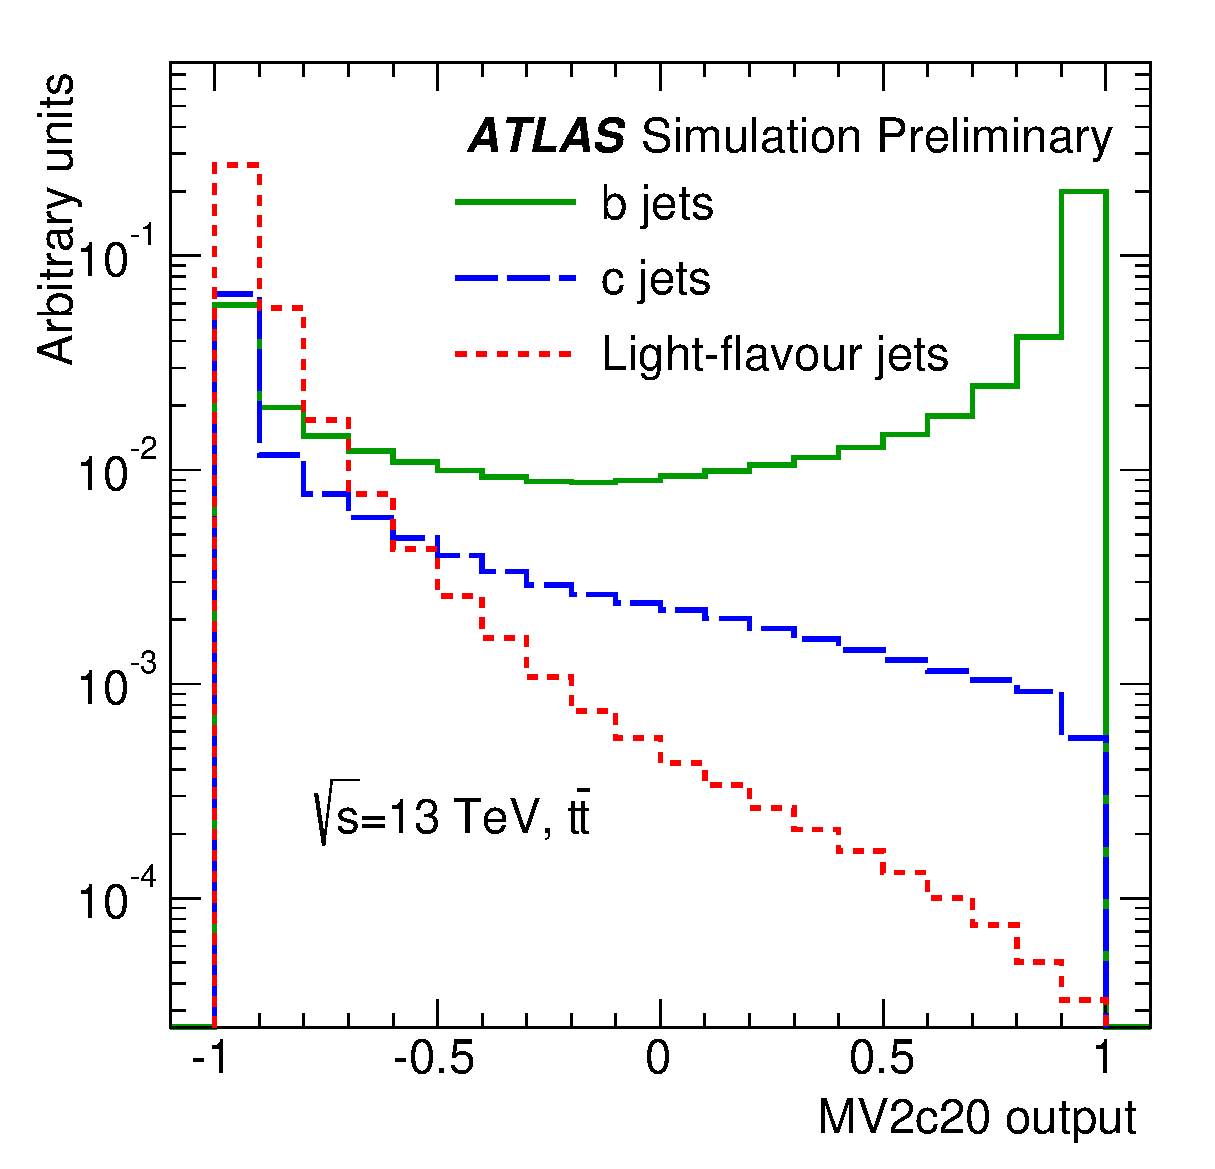
\includegraphics[width=.9\linewidth]{figures/reco/fig_08.eps}
\caption{ Distribution of \texttt{MV2c20} output for $b$-jets, $c$-jets, and light-flavor jets \cite{ATL-PHYS-PUB-2015-022}. }
\label{fig:reco_mv2}
\end{figure}
\end{centering}

\section{Overlap Removal}
\label{sec:reco_or}



\section{Missing Transverse Energy}
\label{sec:reco_met}

Another common usage is $E_T^{miss}$, which gives the negative vectorial sum of the energy in an event. 



